\chapter{Architecture and Design}
\label{chap:architecture_design}
This chapter describes the application scenario in section \ref{sec:scenario_definition} and provides an overview of the system architecture in section \ref{sec:overview}.

\section{Scenario Definition and Goal}
\label{sec:scenario_definition}
This project is designed for a scenario involving the transportation of sensitive pieces of artwork from one place to another. More specifically a \textit{sender} is handing custody of the artwork to a \textit{carrier} who is responsible to transport the artwork safely to a \textit{recipient}. This means the \textit{carrier} is responsible for controlling the transportation environment such that any damages can be prevented. Upon arrival, the artwork's custody is transferred to the \textit{recipient}, and the process is finished.

\begin{figure}[ht]
    \label{fig:scenario}
    \centering
    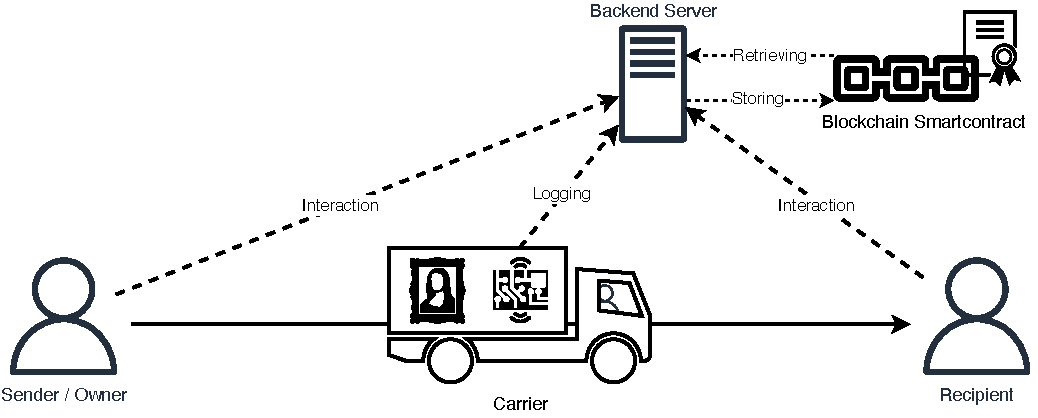
\includegraphics[width=0.8\textwidth]{diagrams/scenario.drawio.pdf}
    \caption{Defined scenario for the system to consider}
\end{figure}

The \textit{sender} of the artwork registers the artwork on the system and inputs relevant information to the application. The system returns an artwork identifier which can be used to retrieve details about the artwork. Before the item is handed over for transportation, the \textit{sender} registers the \textit{carrier} and the \textit{recipient} by adding their corresponding wallet addresses to the system. This allows the other actors to retrieve details about the artwork and interact with the system. A logging device is also registered in the same manner which records and stores environmental data, specifically temperature and humidity, during transportation to be audited by the actors. The logger is set up with a defined threshold specific to the artwork. It will report any violation of this threshold to the system automatically. Once the actors are registered and the logger is set up, both the \textit{carrier} and the \textit{sender} must verify the integrity of the artwork and initiate the request for a status change to "in transit". After which the \textit{carrier} will transport the artwork to its destination where the integrity of the artwork is verified by both the \textit{carrier} and \textit{recipient} and the status is changed to "delivered". If any violation occurred during the transportation the timestamp of the most recent one will be visible for all associated actors in the system.

\subsection*{Goal}
The goal is to create a minimal working system for artwork tracking, considering the following abstractions and the defined scenario. The system should allow the creation of an \gls{nft} associated with a piece of artwork as well as the storing, and retrieval of data on the \gls{nft}. The actors are able to interact with the \gls{sc} via a \gls{rest} \gls{api} that is hosted on the internet. This \gls{api} provides an abstracted form of interaction that does not need a low-level understanding of the underlying blockchain components. Additionally, the system includes a logging device that is programmed to record humidity and temperature data and report any deviations of a predefined threshold to the \gls{api}. Finally, the system should provide a user interface that allows actors to log in with their Ethereum account and interact with the system.

\subsection*{Summary of Abstractions}
The real-world scenario of transferring custody of artwork for transportation is naturally much more complex and involves more actors \cite{artintransit}. However, in this work we are making the following abstractions:
\begin{itemize}
    \item The sender of a specific artwork is also the owner of the artwork
    \item When considering the transportation of the artwork back to the location of origin, the \textit{sender} and \textit{recipient} are the same.
    \item Only temperature and humidity data is recorded by the logger
    \item The authenticity and integrity of the artwork can be verified by any of the actors
\end{itemize}



\section{Overview}
\label{sec:overview}
Since the system is considering a very specific scenario This chapter aims to provide a high-level overview of the architecture of the system while later going into detail about its components and actors. From now on we will call the artwork tracking system \texttt{ARTIS}.

\begin{figure}[ht]
    \centering
    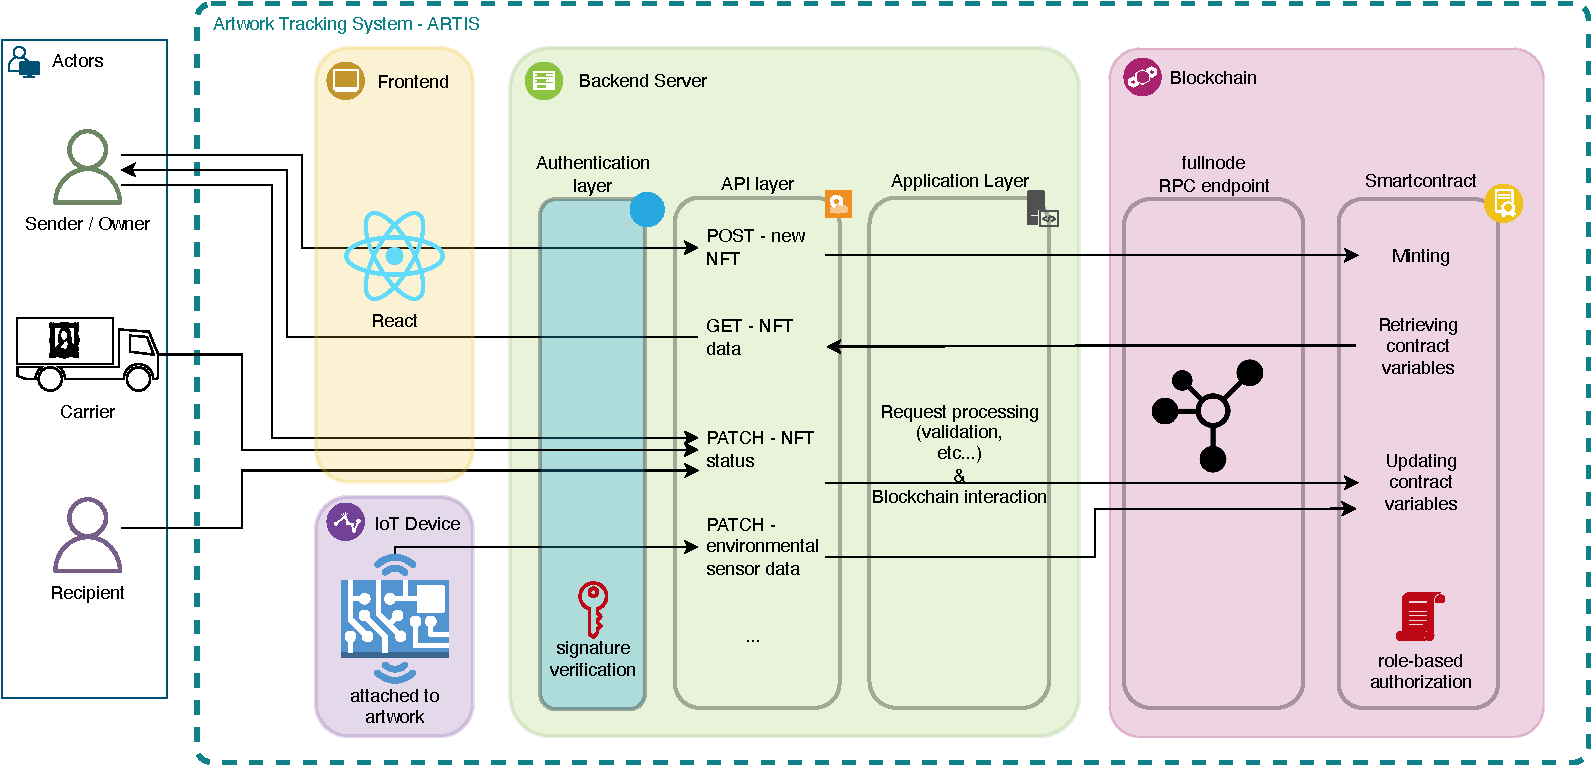
\includegraphics[width=\textwidth, keepaspectratio]{diagrams/architecture.drawio.pdf}
    \caption{System Architecture}
    \label{fig:architecture}
\end{figure}

This architecture was designed using a top-down design approach, with the initial step of building a server application that is able to interact with the \gls{sc}. In the implementation phase, we then added the specific functionality that is needed to support the defined scenario. In Figure \ref{fig:architecture} you can see the final architecture of the system. 

\subsection{Actors}
As already introduced in the section \nameref{sec:scenario_definition}, the system is designed for three actors. Each of the actors is represented by an Ethereum account which is used for authentication and authorization. The actors are defined as follows.

\begin{itemize}[align=left, font=\itshape]
    \item[Sender:] A person or institution that is in charge of dispatching the artwork from a departure location to a destination. This Actor is also considered the \textit{owner} of the artwork. In this context, they can be used interchangeably. The responsibilities of this actor include the initial registration of the artwork as an \gls{nft}, the holding of the \gls{nft} in their \gls{wallet}, and the setup of the \gls{iot} device.

    \item[Carrier:] A transportation company responsible for the safe transport of artwork from one location to another. The \textit{carrier} is committed to delivering the artwork without any damage or alteration. They are also responsible to verify the integrity of the artwork and the logger together with the \textit{sender} and \textit{recipient} upon departure and arrival respectively.

    \item[Recipient:] A person or institution that is receiving the artwork. They share the responsibilities of the \textit{carrier} to verify the integrity of the artwork upon arrival. 
\end{itemize}

\subsection{Technical Components}
Apart from the specified external actors of the system, there are also technical components to consider. The main components of the system are visually separated by colored areas in Figure \ref{fig:architecture}.

\subsubsection{Blockchain}
The blockchain component of the system consists of two sub-components. To interact with the blockchain a \gls{rpc} endpoint is needed. This endpoint can be used by the backend server to submit transactions that are used to interact with the \gls{sc}. For this project, we will consume a managed service to access the Ethereum network and not run our own Ethereum node.

The second component is the \gls{sc} itself. It will be in charge of defining the \gls{nft} of the artwork. 
The functionality provided by the \gls{sc} is defined as follows:

\begin{itemize}[align=left, font=\textit]
    \item[minting:] A new user can create a \gls{nft} of their artwork by entering relevant information about the artwork and the outstanding transportation process.
    \item[retrieving data:] Users are able to retrieve stored data from the \gls{sc}.
    \item[updating data:] Users can update the stored data.
\end{itemize}

The \gls{sc} enforces a role-based authorization that controls the available permission sets of each user. Specifically, this means read access will be granted to \textit{carriers} and \textit{recipients}, while write access, is reserved for the \textit{owner}. It will also handle the multi-approval process necessary for updating the status and changing custody upon transportation of the artwork. An overview of the available permission sets of each actor can be found in Table \ref{tab:permission_sets}

\begin{table}
\begin{tabular}{l|ccccc}
\textbf{Function}          & \textbf{unregistered} & \textbf{owner}       & \textbf{recipient}   & \textbf{carrier}     & \textbf{logger}      \\ \hline
                           & \multicolumn{1}{l}{}  & \multicolumn{1}{l}{} & \multicolumn{1}{l}{} & \multicolumn{1}{l}{} & \multicolumn{1}{l}{} \\
Get artwork data           & ✗                     & ✓                    & ✓                    & ✓                    & ✗                    \\
Update roles               & ✗                     & ✓                    & ✗                    & ✗                    & ✗                    \\
Update violation timestamp & ✗                     & ✗                    & ✗                    & ✗                    & ✓                    \\
Update requested status    & ✗                     & ✓                    & ✓                    & ✓                    & ✗                    \\
Update current Status      & ✗                     & ✗                    & ✗                    & ✗                    & ✗                    \\
Update data fields         & ✗                     & ✓                    & ✗                    & ✗                    & ✗                   
\end{tabular}
\caption{Available permission sets to registered roles}
\label{tab:permission_sets}
\end{table}

\subsubsection{Backend Server}
The backend server is designed to provide an abstracted form of interaction to the \gls{sc} by exposing a \gls{rest} \gls{api}. Like the actors and the logger, the backend server is also represented by an Ethereum account. This account is used to deploy the \gls{sc} and acts as the sole point of access to it. Every transaction is issued by this account. The backend server is also responsible for handling authentication which is designed to prove that incoming requests are made by the actors who are owners of the Ethereum accounts associated with certain roles.

\paragraph{Authentication}
\label{sec:authentication}

\begin{figure}[h]
    \centering
    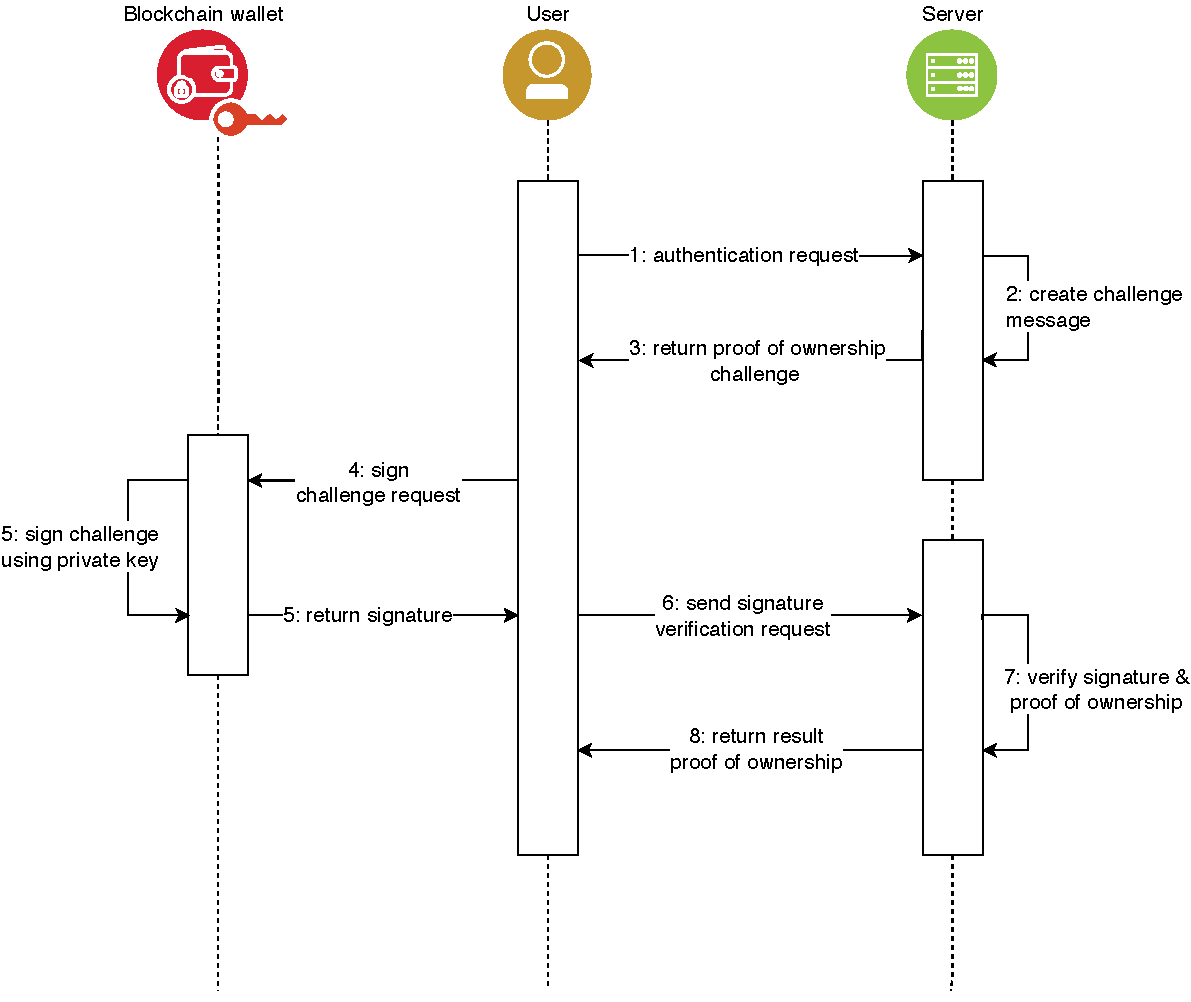
\includegraphics[width=0.59\textwidth, keepaspectratio]{diagrams/authentication_flow.drawio.pdf}
    \caption{Authentication flow}
    \label{fig:auth_flow}
\end{figure}

The authentication flow visualized in Figure \ref{fig:auth_flow} is using signature verification of cryptographically signed messages to prove ownership over an Ethereum account. To do this a challenge message is generated upon authentication request. This message contains relevant information to the session such as the start of the session, the duration of the session, and for which account the session is created. The message is then signed by the private key of the requester's wallet and sent back. The signature can then be verified against the recovered address and if the requested address and recovered address match, this proves that the request was made by an actor who is the owner of the private key corresponding to the account, assuming that the private key was not compromised.

\paragraph{Features}
In addition to enabling the features of the \gls{sc}, and managing authentication, the server will also validate incoming requests and provide meaningful error messages to the user.

\subsubsection{IoT Device}
The logging device is responsible for recording temperature and humidity data while the artwork is in transit. It will evaluate the data against a predefined threshold and report any violation to the system. It will interact with the system via the \gls{api} provided by the backend server. It will not interact with the \gls{sc} directly. However, the logger is also represented by an Ethereum account and equipped with a key pair. This will be used for authentication by signing a message.

\subsubsection{Frontend}
To simplify the interaction with the system we included a user interface in the system. The frontend presentation layer is a web application that is specially designed to simplify the authentication flow by integrating popular blockchain wallets to sign messages and allow the login with wallet functionality. Therefore it should afford to easily guide the user through the authentication flow and provide a graphical interface to the backend server \gls{api}.
